\documentclass[a4paper,% DIN A4-Papier
			12pt, 		% 12er Schrift
			DIV=calc, 	% Seitenränder optimieren
			oneside, 	% einseitiges "Buch"
			headsepline, 	% Trennlinie unter dem Seitenkopf
			ngerman, 	% deutscher Text
			smallheadings, 	% kleinere Überschriften 
			openany, 	% neue Kapitel fangen auf einer neuen freien Seite an
			liststotoc, 	% Verzeichnisse kommen ins Inhaltsverzeichnis
			bibtotoc]	% Literaturverzeichnis kommt ins Inhaltsverzeichnis
			{scrbook} 	% KOMA-Klasse "Buch"
%%%%%%%%%%%%%%%%%%%%%%%%%%%%%%%%%%%%%%%
\input{/home/produnis/Dokumente/LaTeX/src/produnis-src}		% alle meine LaTeX-Befehle
\usepackage{bbding}
%\usepackage[numbers,round]{natbib}
\setlength{\parindent}{0mm}

%
\pdfinfo{/Title FreeQDA - Manual}  % PDF-Info
%
%%%%%%%%%%%%%%%%%%%%%%%%%%%%%%%%%%%%%%%%
%%%%%%%%%%%%%%%%%%%%%%%%%%%%%%%%%%%%%%%%
\begin{document}
\input{/home/produnis/Dokumente/LaTeX/src/mintedSRC}
\bibliographystyle{/home/produnis/Dokumente/LaTeX/src/bmc_article}	% verwendet den natbib-Literaturstyle
%\bibliographystyle{alphadin}

\shorthandoff{"}			% aus "A wird NICHT Ä!
	
%%%%%%%%%%%%%%%%%%%%%%  D E C K B L A T T
%================================================
\begin{titlepage}

\begin{center}


% Upper part of the page
\textsc{\LARGE FreeQDA}\\[1.5cm]
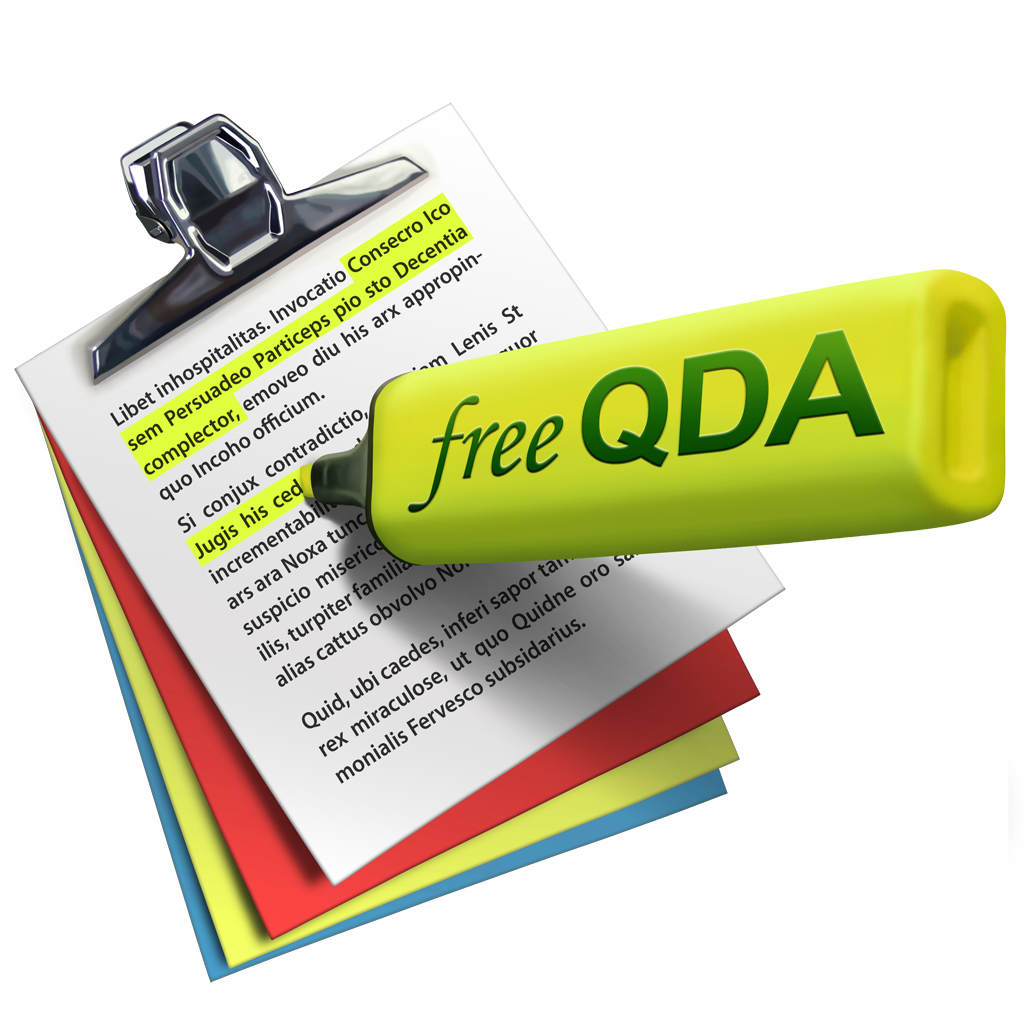
\includegraphics[width=0.25\textwidth]{img/freeQDA_FINAL_1024}\\[1cm]    



\textsc{\Large Eine freie Software zur Analyse \\qualitativer Forschungsdaten}\\[0.5cm]


% Title
\HRule \\[0.4cm]
{ \huge \bfseries Anleitung}\\[0.4cm]

\HRule \\[1.9cm]

% Author and supervisor
%\vfill
\begin{minipage}{0.4\textwidth}
\begin{flushleft} \large
\emph{von}\\
Jörg \textsc{große Schlarmann}
\end{flushleft}
\end{minipage}
\begin{minipage}{0.4\textwidth}
\begin{flushright} \large
\emph{und} \\
Dirk \textsc{Kitscha}
\end{flushright}
\end{minipage}

\vfill

% Bottom of the page
{\large Version vom \today}

\end{center}

\end{titlepage}

%%%%%%%%%%%%%%  V O R S P A N N
%------------------------------------------------------------
\frontmatter  % dies leitet einführende Seiten ein. Die Seitenzahlen werden römisch angezeigt
\chapter{Über FreeQDA}
FreeQDA ist ein freies open-source Softwareprojekt zur Analyse qualitativer Forschungsdaten.


\begin{table}[!h]
\centering
\begin{tabular}{p{30mm}p{40mm}|p{60mm}}
%\textbf{trallala} & \textbf{juppida} \\
\multirow{5}{*}{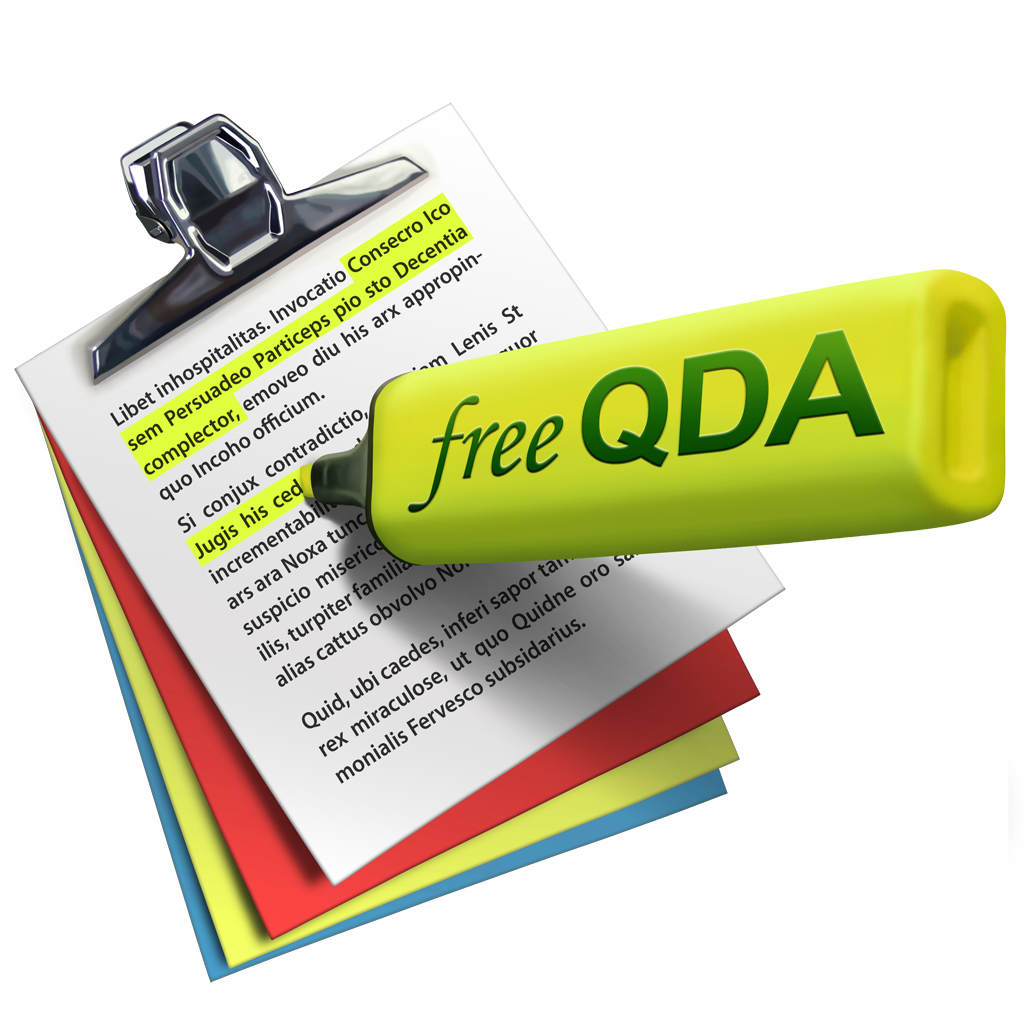
\includegraphics[width=25mm]{img/freeQDA_FINAL_1024}} & \textbf{Programmierung} & Dirk Kitscha	\\
&\textbf{Konzept} & Jörg große Schlarmann	\\
&\textbf{Beratung} & André Fringer		\\
&\textbf{Homepage} & \url{http://freeqda.sf.net} \\
&\textbf{Lizenz} & \href{http://www.gnu.org/licenses/gpl-2.0.html}{GPL 2.0}		\\
\end{tabular}
%\caption{Über FreeQDA}
\label{tab:about}
\end{table}
\vfill
FreeQDA ist freie Software und darf unter den Bedingungen der \href{http://www.gnu.org/licenses/gpl-2.0.html}{GPL 2.0} %
frei verwendet, kopiert und weiterentwickelt werden.\\
Die Entwicklung von FreeQDA wurde von der \textit{Deutschen Gesellschaft für Pflegewissenschaft e.V.}\footnote{\url{http://www.dg-pflegewissenschaft.de}} %
(DGP) gefördert.
\vfill
%----
\tableofcontents	% Inhaltsverzeichnis ausgeben

%%%%%%%%%%%%%% H A U P T T E I L
%-----------------------------------------------------------
\mainmatter   % dies leitet den Haupttext ein. Die Seitenzahlen werden arabisch angezeigt
\include{include/de-start}
\chapter{Installation}

\chapter{Projekte}
FreeQDA arbeitet in so genannten Projekten. Innerhalb eines Projektes können verschiedene Texte und Codes angelegt, gespeichert, verwaltet und %
bearbeitet werden.


\section{Ein neues Projekt beginnen}
\begin{wrapfigure}[9]{l}{0.2\textwidth}
 \vspace{-28pt}
 \begin{center}
    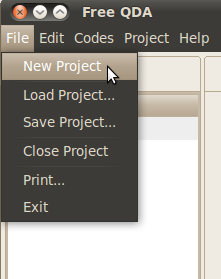
\includegraphics[width=0.18\textwidth]{img/newproject}
  \end{center}
 
%  \caption{Bereich von 2 Standard\-abweich\-ungen}
%  \label{fig:normal3}
  \vspace{12pt}
\end{wrapfigure}
Klicken Sie im Programm-Menü auf \texttt{File => New Project}. Es öffnet sich ein neues Fenster, in welchem Sie gebeten werden, den %
Namen des neuen Projektes einzugeben (siehe Abbildung \ref{fig:newproject}). Geben Sie einen Namen ein (z.B. ``Forschungsprojekt A123'') %
und klicken Sie anschließend auf \texttt{Finish}. Das neues Projekt wird hierdurch erstellt. 

Alle Projekte werden standardmäßig im Programmordner \texttt{FreeQDA/FQDAWorkspace} ab\-ge\-speichert. %In unserem Beispiel 
Jedes Projekt besitzt hier wiederum einen eigenen \textit{Projektordner} (in diesem Beispiel \texttt{Forschungs\-projekt A123}), welcher alle Dateien und Codes %
des Projekts enthält. Die eigentliche Projekt\-hauptdatei liegt auch in diesem Ordner und heisst immer \texttt{project.fqd} (siehe %
Abbildung \ref{fig:projektdatei}).
% 
\begin{figure}[!hbt]
\begin{minipage}[!hb!]{0.5\textwidth}
	\centering
	 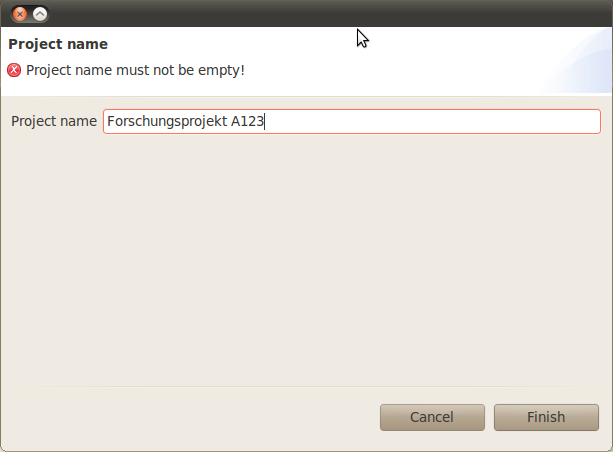
\includegraphics[width=\textwidth]{img/NewProject}
	\caption{Starten Sie ein neues Projekt}
	\label{fig:newproject}
\end{minipage}
\hfill
\begin{minipage}[!hb!]{0.5\textwidth}
	\centering
	 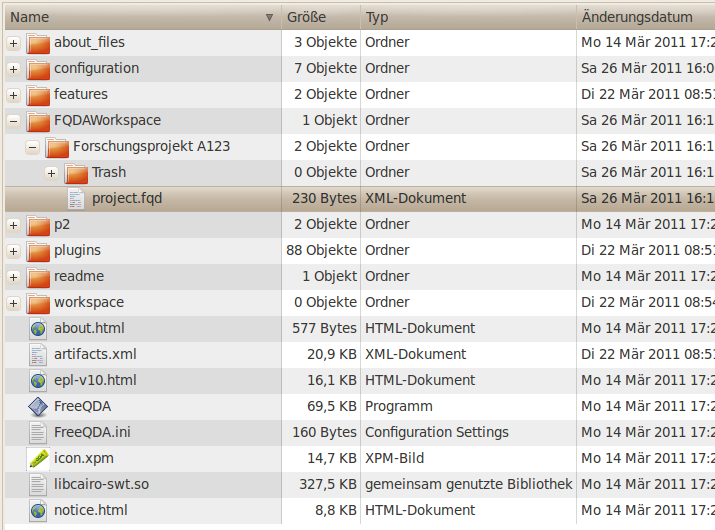
\includegraphics[width=\textwidth]{img/ProjektFile}
	\caption{Projektordner und -datei}
	\label{fig:projektdatei}
\end{minipage}
\end{figure}


\section {Ein Projekt laden}
\begin{wrapfigure}[9]{l}{0.2\textwidth}
 \vspace{-28pt}
 \begin{center}
    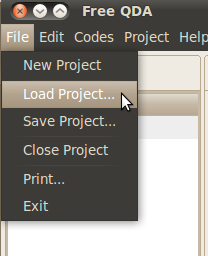
\includegraphics[width=0.18\textwidth]{img/loadproject}
  \end{center}
 
%  \caption{Bereich von 2 Standard\-abweich\-ungen}
%  \label{fig:normal3}
  \vspace{12pt}
\end{wrapfigure}
Um ein bereits vorhandenes Projekt zu laden, klicken Sie im Programm-Menü auf \texttt{File => Load Project}. Es öffnet sich ein %
Dateidialog, in welchem Sie gebeten werden, die gewünschte Projektdatei auszuwählen. Navigieren Sie zunächst in den Ordner %
\texttt{FQDAWorkspace}. Hier werden Ihnen alle vorhandenen Projektordner aufgelistet. Klicken Sie nun doppelt auf den gewünschten Ordner %
und wählen Sie die Projektdatei \texttt{project.fqd} aus. Bestätigen Sie durch einen Klick auf den \texttt{OK} Button Ihre Auswahl. %
Das Projekt wird nun geladen.



\chapter{Texte}
Innerhalb eines Projekts können Sie beliebig Texte anlegen und verwalten. Hierfür steht Ihnen der \texttt{Projekt Browser} %
zur Verfügung, den Sie im oberen Teil der Navigationsleiste finden (siehe Abbildung \ref{fig:projectbrowser}).

\section{Texte hinzufügen}
\label{sec:newtext}
% 
Um einen neuen Text hinzuzufügen, klicken Sie in der Menüleiste auf \texttt{Project => Create new text} (Abbildung \ref{fig:texthinzu}). %
Alternativ können Sie auch den Mauszeiger über den Project Browser führen und dann die rechte Maustaste klicken.  %

\begin{figure}[!hbt]
\begin{minipage}[!hb!]{0.5\textwidth}
	\centering
	 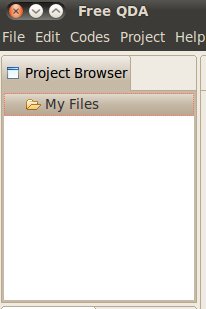
\includegraphics[width=0.5\textwidth]{img/ProjectBrowser}
	\caption{Project Browser}
	\label{fig:projectbrowser}
\end{minipage}
\hfill
\begin{minipage}[!hb!]{0.5\textwidth}
	\centering
	 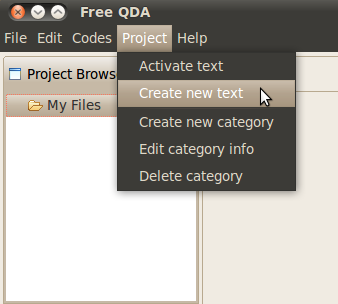
\includegraphics[width=0.8\textwidth]{img/CreateNewText}
	\caption{Text hinzufügen}
	\label{fig:texthinzu}
\end{minipage}
\end{figure}

Es öffnet sich ein neues Fenster, in welchem Sie gebeten werden, den Namen des neuen Textes einzugeben (Abbildung \ref{fig:neuertext1}). %
Geben Sie den Namen ein und klicken Sie \texttt{Finish}. Der neue Text erscheint nun im Project Browser (Abbildung \ref{fig:neuertext2}). 
Durch einen Doppelklick auf den Textnamen öffnen Sie den neuen Text im Editor. Innerhalb des Editors können Sie nun Ihren neuen Text %
schreiben. 
\begin{figure}[!hbt]
\begin{minipage}[!hb!]{0.5\textwidth}
	\centering
	 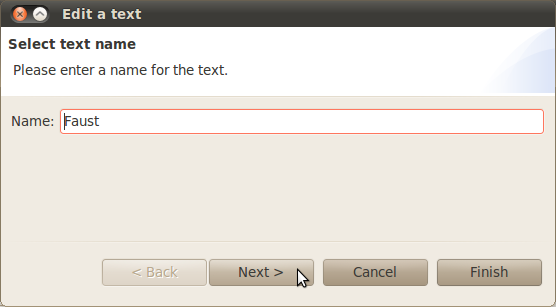
\includegraphics[width=0.8\textwidth]{img/NexText}
	\caption{Textname eingeben}
	\label{fig:neuertext1}
\end{minipage}
\hfill
\begin{minipage}[!hb!]{0.5\textwidth}
	\centering
	 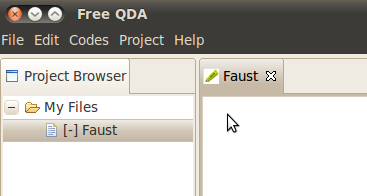
\includegraphics[width=0.8\textwidth]{img/NewText2}
	\caption{Text hinzufügen}
	\label{fig:neuertext2}
\end{minipage}
\end{figure}

Wenn Sie einen Text aus einer bereits bestehenden Datei (z.B. doc, txt, rtf, odt) übernehmen möchten, müssen Sie diese Datei im jeweiligen %
Programm (Word, LibreOffice, etc) öffnen, den gesamten Text dort markieren und in die Zwischenablage kopieren. Jetzt können Sie zum %
FreeQDA-Editor zurückkehren, und den Text mit der Tastenkombination \texttt{STR} und \texttt{V} (bzw. am Mac per  \texttt{APFEL} %
und \texttt{V}) einfügen. 
\begin{figure}[!htb]
	\centering
	 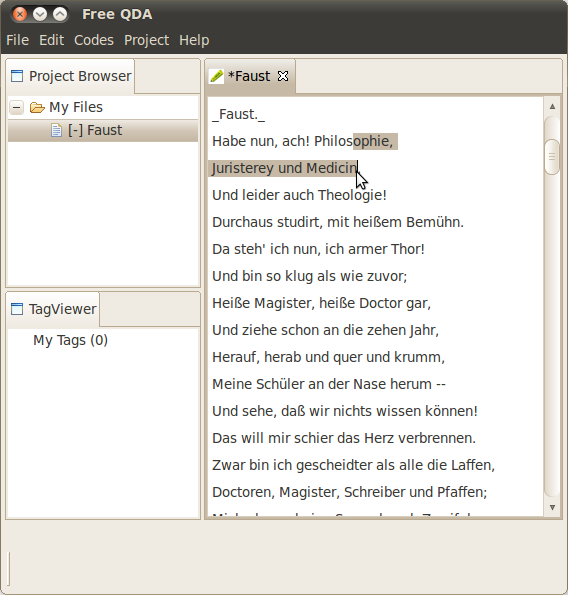
\includegraphics[width=0.4\textwidth]{img/Faust1}
	\caption{Text im Editor}
	\label{fig:faust}
\end{figure}
\vfill

Um den Texteditor zu schließen, klicken Sie in der Tableiste auf das $\times$ Symbol neben dem Textnamen (Abbildung \ref{fig:textschliessen}). %
Das * Symbol vor dem Textnamen (siehe Abbildung \ref{fig:textschliessen} *Faust) bedeutet, dass an dem Text Änderungen vorgenommen wurden, %
die noch nicht gespeichert sind. Wenn Sie den Texteditor schließen, werden Sie daher gefragt, ob Ihre Änderungen gespeichert werden sollen. %
Bestätigen Sie mit \texttt{Yes} um den Text zu speichern. Alle Texte werden übrigens mit der Dateiendung \texttt{fqf} im Projektordner gespeichert (Abbildung \ref{fig:textdatei}). %
Sie sollten diese jedoch nicht mit einem anderen Programm öffnen, da FreeQDA innerhalb der Texte weitere Informationen speichert, welche %
durch andere Programme evtl. überschrieben werden. 
\vfill
\begin{figure}[!hbt]
\begin{minipage}[!hb!]{0.5\textwidth}
	\centering
	 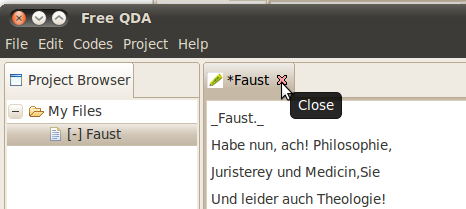
\includegraphics[width=0.8\textwidth]{img/TextSchliessen}
	\caption{Text schließen}
	\label{fig:textschliessen}
\end{minipage}
\hfill
\begin{minipage}[!hb!]{0.5\textwidth}
	\centering
	 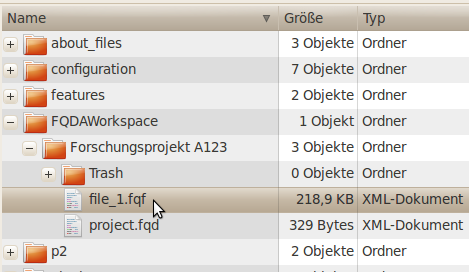
\includegraphics[width=0.7\textwidth]{img/textdatei}
	\caption{Textdatei}
	\label{fig:textdatei}
\end{minipage}
\end{figure}
\newpage
\section{Einen Text löschen}
Um einen Text zu löschen klicken Sie im Project Browser mit der rechten Maustaste auf den gewünschten Text und wählen Sie %
\texttt{Delete Text} (siehe Abbildung \ref{fig:deletetext}).

\begin{figure}[!htb]
	\centering
	 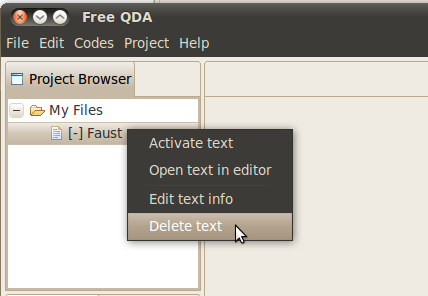
\includegraphics[width=0.4\textwidth]{img/deletetext}
	\caption{Text löschen}
	\label{fig:deletetext}
\end{figure}


\section{Textkategorien}
\label{sec:textcategory}
Texte können in beliebigen Textkategorien verwaltet werden. Um eine neue Textkategorie zu erstellen, klicken Sie in der Menüleiste auf %
\texttt{Project => Create new category} (Abbildung \ref{fig:createnewcategory}). Alternativ können Sie auch innerhalb des Project Browser %
auf die rechte Maustaste klicken. Es öffnet sich ein neues Fenster, in welchem Sie gebeten werden, den Namen der neuen Kategorie %
einzutippen (Abbildung \ref{fig:newcategoryname}). Geben Sie den gewünschten Namen ein und klicken Sie auf \texttt{Finish}. Die neue Kategorie ist nun erstellt.

\begin{figure}[!hbt]
\begin{minipage}[!hb!]{0.42\textwidth}\scriptsize
	\centering
	 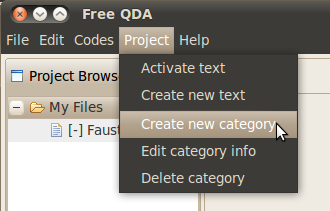
\includegraphics[width=0.7\textwidth]{img/createnewcategory}
	\caption{Textkategorie erstellen}
	\label{fig:createnewcategory}
\end{minipage}
\hfill
\begin{minipage}[!hb!]{0.41\textwidth}
	\centering
	 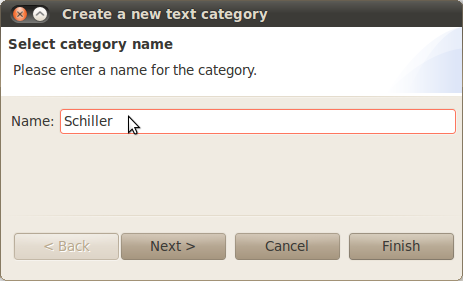
\includegraphics[width=0.75\textwidth]{img/newcategoryname}
	\caption{Kategorie benennen}
	\label{fig:newcategoryname}
\end{minipage}
\hfill
\begin{minipage}[!hb!]{0.15\textwidth}
	\centering \vspace{-26pt}
	 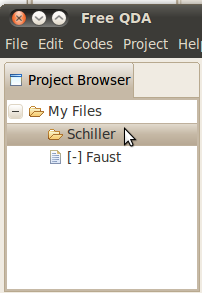
\includegraphics[width=0.9\textwidth]{img/newcategory2}
%	\caption{neue Kategorie}
	\label{fig:newcategory2}
\end{minipage}
\end{figure}


\subsection{Einer Kategorie einen neuen Text hinzufügen}
\begin{wrapfigure}[10]{l}{0.5\textwidth}
 \vspace{-28pt}
 \begin{center}
    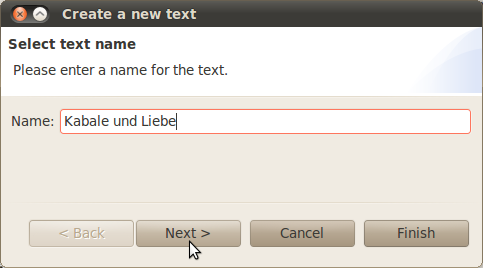
\includegraphics[width=0.45\textwidth]{img/createnewtext3}
  \end{center}
 
	\caption{Klicken Sie auf \texttt{Next}}
	\label{fig:newtext3}
  \vspace{12pt}
\end{wrapfigure}

Um einer Kategorie einen neuen Text hinzuzufügen gehen Sie ähnlich vor wie auf Seite \pageref{sec:newtext}. %  
Klicken Sie im Menü auf \texttt{Project => Create new text}. Es öffnet sich ein neues Fenster, in welchem Sie den Namen des neuen Textes eintragen müssen. %
Klicken Anschließend auf den \texttt{Next} Button (\textbf{nicht} auf den \texttt{Finish} Button, siehe Mauszeiger in Abbildung \ref{fig:newtext3}). Es wird Ihnen nun %
die aktuelle Kategoriestruktur der Texte angezeigt. 
%
\begin{wrapfigure}[12]{l}{0.5\textwidth}
 \vspace{-15pt}
 \begin{center}
    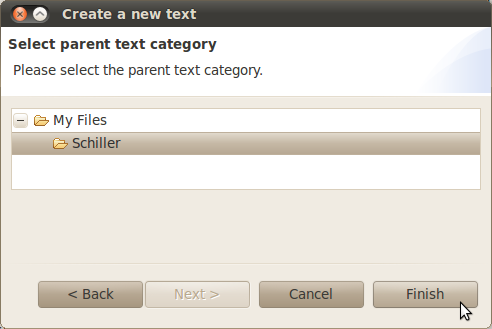
\includegraphics[width=0.45\textwidth]{img/createnewtext4}
	\caption{Kategorie auswählen}
	\label{fig:newtext4}
  \end{center}
  \vspace{12pt}
\end{wrapfigure}
% 
% \begin{figure}[!hbt]
% \begin{minipage}[!hb!]{0.5\textwidth}
% 	\centering
% 	 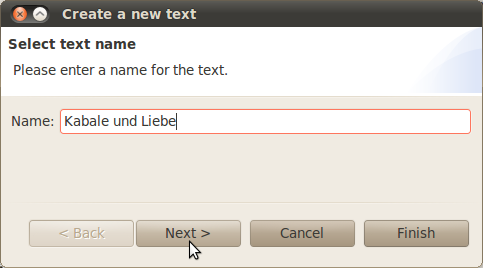
\includegraphics[width=0.8\textwidth]{img/createnewtext3}
% 	\caption{Klicken Sie auf \texttt{Next}}
% 	\label{fig:newtext3}
% \end{minipage}
% \hfill
% \begin{minipage}[!hb!]{0.5\textwidth}
% 	\centering
% 	 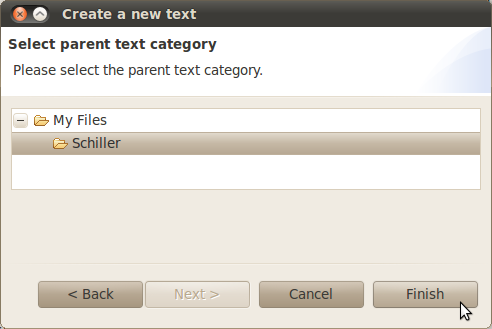
\includegraphics[width=0.7\textwidth]{img/createnewtext4}
% 	\caption{Kategorie auswählen}
% 	\label{fig:newtext4}
% \end{minipage}
% \end{figure}
% 

In unserem Beispiel existiert nur der Ordner \textit{Schiller} (Abbildung \ref{fig:newtext4}). %
Klicken Sie auf den gewünschten Ordner und anschließend auf den \texttt{Finish} Button. 


Die neue Textdatei ist nun im Project Browser unter der genannten Kategorie verfügbar (Abbildung \ref{fig:newtext5}). %
Klicken Sie doppelt auf die Textdatei um den Text im Editor zu öffnen. Innerhalb des Editors können Sie Text %
schreiben oder aus der Zwischenablage einfügen. In Abbildung \ref{fig:newtext5} wurde der Text \textit{Kabale und Liebe} per copy und paste von einer Webseite in den %
Editor übertragen.

Im Project Browser sind alle Kategorien und Texte aufgelistet. Durch Doppelklick auf einen gewünschten Text %
öffnen Sie diesen im Editor. Alle Datein die derzeit im Editor geöffnet sind werden in der Tableiste angezeigt (Abbildung \ref{fig:texttab}). Durch Klicken auf einen %
Tab wechseln Sie zum gewünschten Text. 
\begin{figure}[!hb]
\begin{minipage}[!hb!]{0.5\textwidth}
	\centering
	 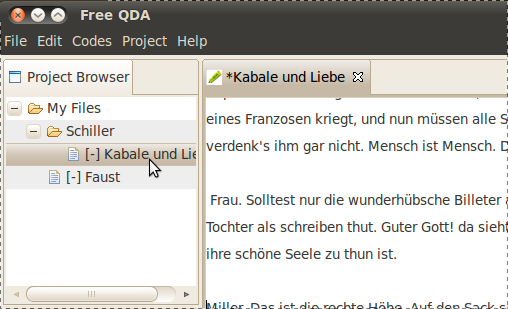
\includegraphics[width=0.75\textwidth]{img/createnewtext5}
	\caption{Textdatei}
	\label{fig:newtext5}
\end{minipage}
\hfill
\begin{minipage}[!hb!]{0.5\textwidth}
	\centering
	 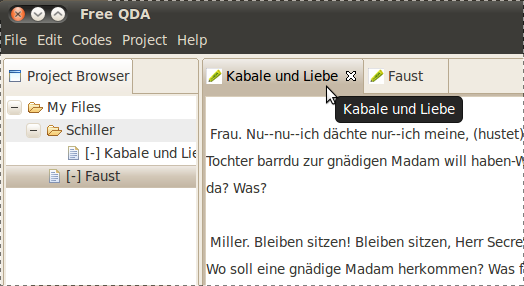
\includegraphics[width=0.8\textwidth]{img/texttab}
	\caption{Texte im Tab}
	\label{fig:texttab}
\end{minipage}
\end{figure}

\chapter{Codes}
\begin{wrapfigure}[7]{l}{0.2\textwidth}
 \vspace{-28pt}
 \begin{center}
    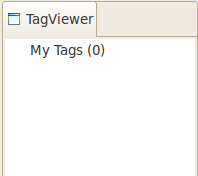
\includegraphics[width=0.18\textwidth]{img/codebrowser}
  \end{center}
  \vspace{12pt}
\end{wrapfigure}
Mit FreeQDA können Passagen aus Texten mit beliebigen Codes (auch \textit{Tag} genannt) markiert werden. Sind alle Texte mit den %
gewünschten Codes versehen, kann FreeQDA für beliebige Codes eine Übersichtsseite erzeugen, auf welcher jene Textstellen aufgelistet werden, die %
mit dem jeweiligen Code markiert wurden. 
Ähnlich wie bei Texten können Codes beliebig in Kategorien sortiert werden. Hierfür steht in der Navigationsleiste der \texttt{TagViewer} %
bereit. Innerhalb des TagViewers werden alle Code-Kategorien und Codes aufgelistet. Wenn Sie ein neues Projekt beginnen, ist diese Liste %
natürlich zunächst leer. 


\section{Einen neuen Code erstellen}
Neue Codes werden ähnlich angelegt wie Texte. Wählen Sie aus dem Programm-Menü den Punkt \texttt{Codes => Create Tag} aus (Abbildung \ref{fig:newtag1}). %
Alternativ können Sie auch %
die Maus über den TagViewer führen und die rechte Maustaste klicken. Es öffnet sich ein neues Fenster, in welchem Sie aufgefordert werden den %
Namen des neuen Codes einzutragen (Abbildung \ref{fig:tagname}). Tragen Sie also den Namen ein und klicken Sie anschließend auf das kleine %
Kästchen neben \texttt{Color}.

\begin{figure}[!hb]
\begin{minipage}[!hb!]{0.5\textwidth}
	\centering
	 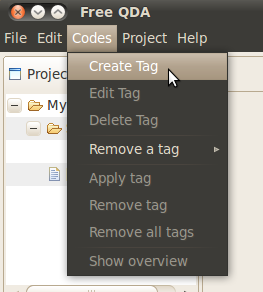
\includegraphics[width=0.42\textwidth]{img/createtag1}
	\caption{Tag erstellen}
	\label{fig:newtag1}
\end{minipage}
\hfill
\begin{minipage}[!hb!]{0.5\textwidth}
	\centering
	 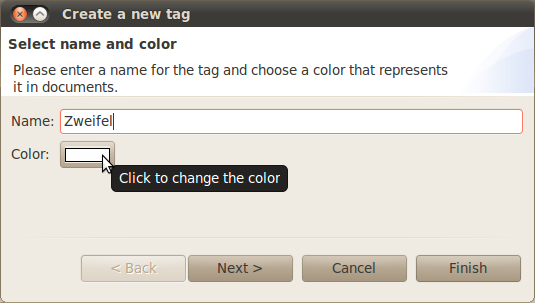
\includegraphics[width=0.8\textwidth]{img/tagname}
	\caption{Name des Tags}
	\label{fig:tagname}
\end{minipage}
\end{figure}

Es öffnet sich nun ein weiteres Fenster, in welchem Sie die gewünschte Code-Farbe auswählen können (Abbildung \ref{fig:tagfarbe1}). %
Mit der Farbe, die Sie hier auswählen, werden die Textstellen, die mit dem Code getaggt werden, farblich hinterlegt. Haben Sie eine Farbe %
gewählt, bestätigen Sie Ihre Auswahl durch Klick auf \texttt{OK}. Die ausgewählte Farbe wird nun auch im Namensfenster des neuen Tags %
angezeigt (Abbildung \ref{fig:tagfarbe2}). Klicken Sie nun auf \texttt{Finish} um den Code zu erzeugen.

\begin{figure}[!hb]
\begin{minipage}[!hb!]{0.5\textwidth}
	\centering
	 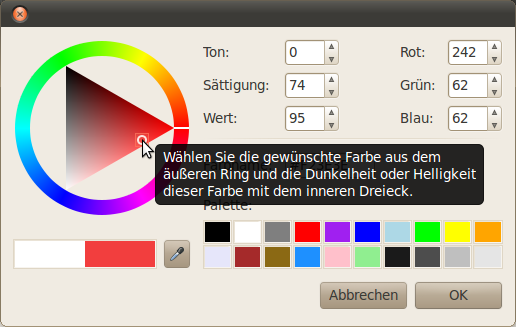
\includegraphics[width=0.5\textwidth]{img/tagfarbe}
	\caption{Tagfarbe auswählen}
	\label{fig:tagfarbe1}
\end{minipage}
\hfill
\begin{minipage}[!hb!]{0.5\textwidth}
	\centering
	 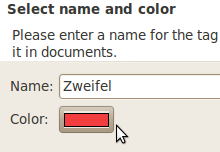
\includegraphics[width=0.45\textwidth]{img/tagfarbe2}
	\caption{Tagfarbe}
	\label{fig:tagfarbe2}
\end{minipage}
\end{figure}

\section{Einen Code unterhalb eines anderen Codes erstellen}
\begin{wrapfigure}[11]{l}{0.5\textwidth}
 \vspace{-28pt}
 \begin{center}
    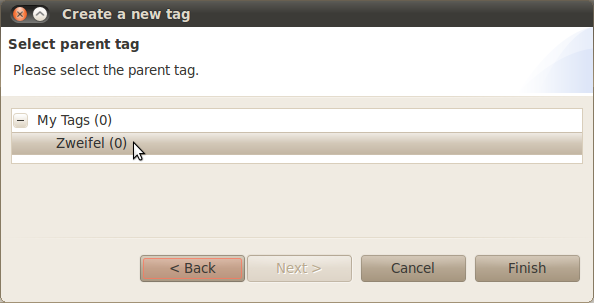
\includegraphics[width=0.48\textwidth]{img/subtag}
	\caption{Tag-Kategorie wählen}
	\label{fig:subtag}
  \end{center}
  \vspace{12pt}
\end{wrapfigure}
Ähnlich wie bei Textkategorien (siehe Seite \pageref{sec:textcategory}), können auch Codes ineinader verschachtelt werden. 
Legen Sie zunächst wie oben beschrieben einen neuen Tag an, indem Sie in der Menüleiste auf \texttt{Codes => Create Tag} klicken. %
Es öffnet sich das Fenster, in welchem Sie den Tagnamen sowie die Farbe auswählen können. Klicken Sie hier auf den \texttt{Next}-Button %
(und \textbf{nicht} auf \texttt{Finish}). Es wird Ihnen nun eine Liste aller vorhandenen Codes angezeigt. Klicken Sie hier auf den %
Code, unterhalb welchen der neue Code angelegt werden soll (Abbildung \ref{fig:subtag}). Bestätigen Sie Ihre Auswahl per %
Klick auf \texttt{Finish}.\\[4mm] %

\begin{wrapfigure}[3]{l}{0.2\textwidth}
 \vspace{-28pt}
 \begin{center}
    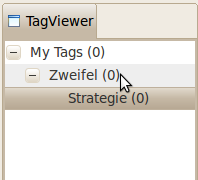
\includegraphics[width=0.18\textwidth]{img/tagviewer}
  \end{center}
  \vspace{12pt}
\end{wrapfigure}

Der neue Code wird nun im TagViewer angezeigt und kann von dort ausgewählt und verwendet werden. In unserem Beispiel wurde der %
Code \textit{Strategie} unterhalb des Codes \textit{Zweifel} angelegt.\\[16mm]
\vfill
\section{Eine Textstelle taggen}
\begin{wrapfigure}[9]{l}{0.4\textwidth}
 \vspace{-28pt}
 \begin{center}
    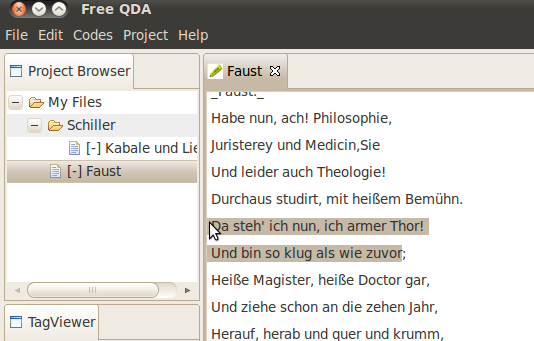
\includegraphics[width=0.38\textwidth]{img/tagtext1}
	\caption{Textstelle markieren}
	\label{fig:texttag1}
  \end{center}
  \vspace{12pt}
\end{wrapfigure}

Eine der Hauptaufgaben von FreeQDA ist es, Textstellen mit beliebigen Codes zu taggen. Um eine Textstelle mit einem Code zu versehen öffnen %
Sie zunächst den gewünschten Text im FreeQDA-Editor. Hierzu führen Sie im Project Browser einen Doppelklick auf den gewünschten Text aus. %
Suchen Sie nun innerhalb des Editors eine passende Textstelle aus, die Sie mit einem Code versehen möchten. Markieren Sie diesen %
Textbereich mit der Maus (siehe Abbildung \ref{fig:texttag1}).

\newpage

\begin{figure}[!hbt]
\begin{minipage}[!hb!]{0.5\textwidth}\scriptsize
	\centering
	 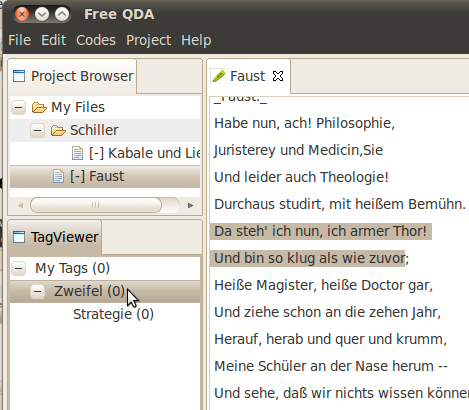
\includegraphics[width=0.7\textwidth]{img/tagtext2}
	\caption{Tag auswählen}
	\label{fig:texttag2}
\end{minipage}
\hfill
\begin{minipage}[!hb!]{0.5\textwidth}
	\centering
	 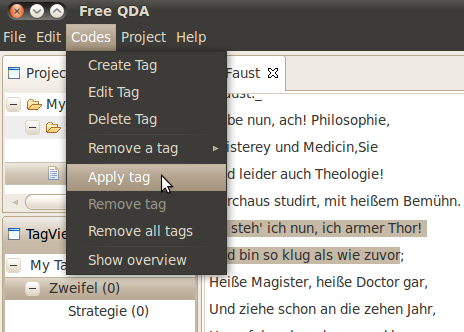
\includegraphics[width=0.8\textwidth]{img/tagtext3}
	\caption{Code setzen}
	\label{fig:texttag3}
\end{minipage}
\end{figure}

Wählen Sie jetzt aus dem TagViewer den gewünschten Code aus (Abbildung \ref{fig:texttag2}). Anschließend wird der Code über den Menüpunkt %
\texttt{Codes => Apply tag} auf die Textstelle angewendet (Abbildung \ref{fig:texttag3}).  Alternativ können Sie auch mit der rechten Maustaste %
auf den gewünschten Code klicken. %
Innerhalb des Editors ist die Textstelle nun mit der Farbe des gesetzten %
Codes unterlegt (Abbildung \ref{fig:texttag4}). Wenn Sie innerhalb des Editors mit der Maus über eine getaggte Textstelle fahren und dort %
etwas warten, werden Ihnen weitere Informationen zu den gesetzten Codes angezeigt. Im Beispiel der Abbildung \ref{fig:texttag4} sehen Sie, %
dass die Textzeilen 843 bis 844 mit dem Code ``\textit{Zweifel}'' getaggt ist.


\begin{figure}[!hbt]
	\centering %\vspace{-26pt}
	 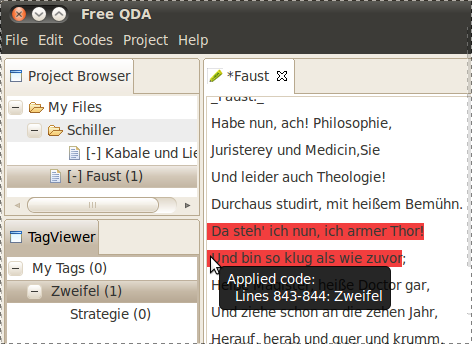
\includegraphics[width=0.5\textwidth]{img/tagtext4}
	\caption{Code im Text}
	\label{fig:texttag4}
\end{figure}

Des Weiteren können Sie sehen, dass in Abbildung \ref{fig:texttag4} sowohl hinter dem Text \textit{Faust} sowie hinter dem Code %
\textit{Zweifel} jeweils eine \texttt{1} angezeigt wird. Dies bedeutet, dass im Text \textit{Faust} insgesamt \textit{eine} kodierte %
Textstelle enthalten ist. Des Weiteren bedeutet es, dass der Code \texttt{Zweifel} insgesamt auf eine Textstelle angewendet wurde. 


\begin{wrapfigure}[4]{l}{0.3\textwidth}
 \vspace{-28pt}
 \begin{center}
    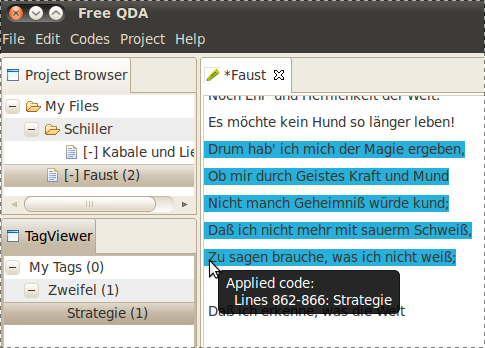
\includegraphics[width=0.28\textwidth]{img/tagtext5}
	\caption{Coden}
	\label{fig:texttag5}
  \end{center}
  \vspace{12pt}
\end{wrapfigure}

Wenn nun ein weitere Code gesetzt wird, erhöht sich die Zahl entsprechend. In Abbildung \ref{fig:texttag5} wurde eine weitere Textstelle des %
\textit{Faust} mit dem Code \textit{Strategie} getaggt. Dementsprechend erhöht sich der Zähler im Project Browser hinter \textit{Faust} %
auf 2.


\newpage
\section{Übersichten erstellen}
Haben Sie Textstellen mit Codes versehen, können Sie sich Übersichten für einzelne Codes in ausgewählten Texten anzeigen lassen. 
Hierfür ist es notwendig, die gewünschten Texte zunächst zu \textit{aktivieren}. Markieren Sie im Project Browser einen gewünschten Text. %
Wählen Sie anschließend aus dem Programm-Menü den Eintrag \texttt{Project => Activate text} (Abbildung \ref{fig:activatetext1}). %
Alternativ können Sie auch mit der rechten Maustaste auf den Text klicken. Einen aktivierten Text erkennen Sie an dem Symbol \texttt{[x]} %
vor dem Textnamen (siehe Mauszeiger in Abbildung \ref{fig:activatetext2}). Auf die selbe Weise können Sie Texte auch wieder de-aktivieren.

\begin{figure}[!hbt]
\begin{minipage}[!hb!]{0.5\textwidth}\scriptsize
	\centering
	 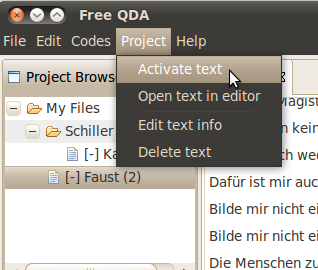
\includegraphics[width=0.7\textwidth]{img/activatetext1}
	\caption{Text aktivieren}
	\label{fig:activatetext1}
\end{minipage}
\hfill
\begin{minipage}[!hb!]{0.5\textwidth}
	\centering
	 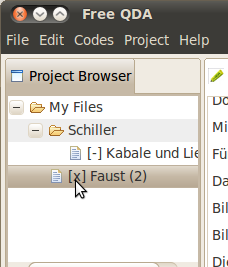
\includegraphics[width=0.5\textwidth]{img/activatetext2}
	\caption{aktivierter Text}
	\label{fig:activatetext2}
\end{minipage}
\end{figure}

Nachdem Sie alle gewünschten Texte aktiviert haben, markieren Sie im TagViewer einen Code, für welchen Sie eine Überischt erstellen möchten. %
Wählen Sie nun aus dem Programm-Menü den Eintrag \texttt{Codes => Show overview} (Abbildung \ref{fig:overview1}). Alternativ können Sie auch %
mit der rechten Maustaste auf den gewünschten Code klicken.

FreeQDA erzeugt nun eine Übersicht aller Textstellen in allen aktivierten Texten, die mit dem ausgewählten Code getaggt wurden (Abbildung \ref{fig:overview2}).
Da wir in unserem Beispiel den Code nur einmal vergeben haben, wird dementsprechend in Abbildung \ref{fig:overview2} auch nur diese eine %
Textstelle angezeigt.

Innerhalb der Überischt können Sie übrigens weitere Textstellen mit beliebigen Codes taggen. Ihre Eingaben werden in den Originaltexten gespeichert.
Natürlich können Sie die Übersichten auch ausdrucken. Wählen Sie hierzu im Programm-Menü den Punkt \texttt{File => Print}.

\begin{figure}[!hbt]
\begin{minipage}[!hb!]{0.5\textwidth}\scriptsize
	\centering
	 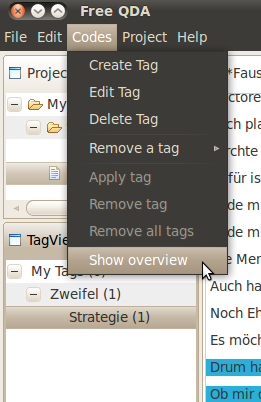
\includegraphics[width=0.4\textwidth]{img/showoverview}
	\caption{Übersicht erzeugen}
	\label{fig:overview1}
\end{minipage}
\hfill
\begin{minipage}[!hb!]{0.5\textwidth}
	\centering
	 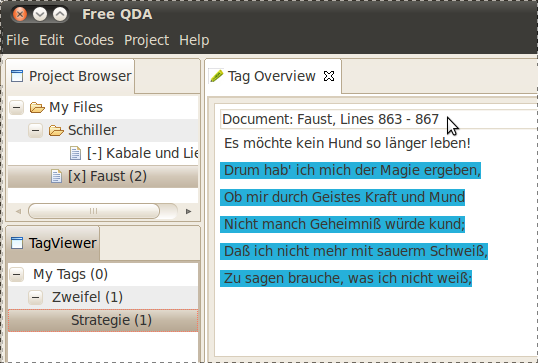
\includegraphics[width=0.9\textwidth]{img/overview1}
	\caption{Übersicht}
	\label{fig:overview2}
\end{minipage}
\end{figure}


%
%
%
%-------------------------------------------------------------------
%\bibliography{../freeqda_manual}
\listoffigures		% beginnend mit dem Abbildungsverzeichnis
\listoftables		%... und dem Tabellenverzeichnis
%\listoflistings		% aus dem minted-Paket
%\newpage
%\printnomenclature	% Abkürzungsverzeichnis ausgeben
%-------------------------
\backmatter    % hiermit wird  der Nachspann eingeleitet. Seitenzahlen werden weiter fortgeführt
%\appendix
%\addcontentsline{toc}{chapter}{Anhang}
% \input{includes/Linkliste}
%\theendnotes
%
%---------------------
\end{document}
%%%%%%%%%%%%%%%%%%%%%%%%%%%%%%%%%%%%%%%%
%%%%%%%%%%%%%%%%%%%%%%%%%%%%%%%%%%%%%%%%
%%%%%%%%%%%%%%%%%%%%%%%%%%%%%%%%%%%%%%%%
%
%%%%% end of file